\documentclass[11pt]{article}
\usepackage[utf8]{inputenc}
\usepackage{mathtools}
\usepackage{vmargin}
\usepackage{graphicx}
\usepackage{lmodern}
\usepackage[T1]{fontenc}
\usepackage{multirow}
\usepackage[noline,ruled,linesnumbered,spanish]{algorithm2e}
\usepackage{forest}
\usepackage{forest,adjustbox}
\usepackage{color}

\setpapersize{A4}
\setmargins{2.5cm}       % margen izquierdo
{0cm}                        % margen superior
{16.5cm}                      % anchura del texto
{23.42cm}                    % altura del texto
{10pt}                           % altura de los encabezados
{1cm}                           % espacio entre el texto y los encabezados
{0pt}                             % altura del pie de página
{2cm}                           % espacio entre el texto y el pie de página

\title{Mini-Proyecto III: Estructuras de Datos Sucintas}
\author{Cristobal Donoso Oliva}
\author{
Diego Seco$^{1}$, Meraioth Ulloa Salazar$^{2}$, Cristóbal Donoso Oliva$^{3}$,\\ Matías Medina Silva$^{4}$,\\ \\
\small{$^{1}$Docente a cargo de la asignatura$^{2-3-4}$Estudiantes Pre-grado}\\
\small{$^{1-2}$Dpto. de Ingeniería Civil Informática y Ciencias de la Computación}\\
\small{Universidad de Concepción, Concepción, Chile.}\\
}
\date{Noviembre de 2016}
\usepackage{amsmath}
\begin{document}

\maketitle


\section{predecesor y sucesor}
\subsection{Descripción del problema}
Se tiene \textbf{t} elementos de un conjunto [1,n] y se quieren hacer dos tipos de consultas sobre dicho conjunto:
\begin{itemize}
\item Sucesor: Dado un número i, ¿Cuál es el menor número $\geq$ i en el conjunto?
\item Predecesor: Dado un número i, ¿Cuál es el mayor número $\leq$ i en el conjunto?
\end{itemize}
Para este problema se proponen dos soluciones usando las siguientes estructuras de datos:
\subsection{Solución BST}
Para poder calcular el predecesor y sucesor de un elemento del BST primero debemos definir el mínimo y máximo elemento en un árbol binario. Los nodos mínimo y máximo de un BST se encontrarían más a la izquierda y más a la derecha respectivamente desde la raíz (ver figura 5 y 6). 
\begin{figure}[htp]
\centering
\begin{minipage}{.4\textwidth}
\centering
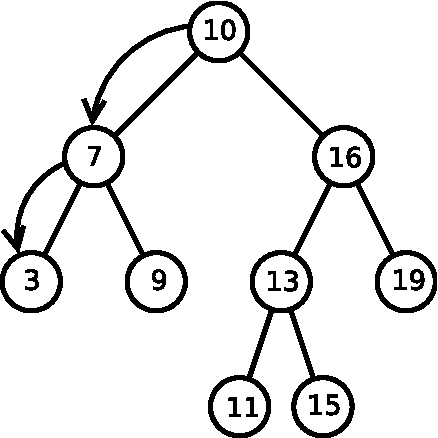
\includegraphics[scale=0.5]{min_arbol.pdf}
\\\scriptsize{\color{white}.\color{black}\\Figura 5: Nodo mínimo en un BST}
\label{etiqueta}
\end{minipage}
\begin{minipage}{.4\textwidth}
\centering
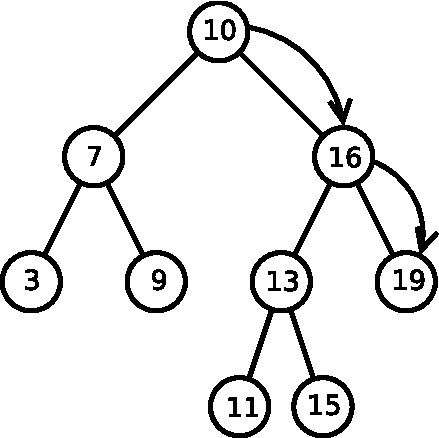
\includegraphics[scale=0.5]{max_arbol.pdf}
\\\scriptsize{\color{white}.\color{black}\\Figura 6: Nodo máximo en un BST}
\label{etiqueta}
\end{minipage}
\end{figure}

Entonces, Para poder encontrar el predecesor y sucesor:
\begin{itemize}
\item Si el nodo i tiene dos hijos su predecesor es el valor máximo en el sub-árbol a la izquierda de i y su sucesor sería el valor mínimo en en el sub-árbol a la derecha de i.
\item Si no entonces:
\begin{itemize}
\item Si i no tiene hijo izquierdo entonces su predecesor es su primer ancestro izquierdo.
\item Si i no tiene hijo derecho entonces su sucesor es su primer ancestro derecho.
\end{itemize}
\end{itemize}
\subsection{Solución Bitmap}
Cada indice del bitmap B representa un elemento de conjunto [1,n], donde un 1 representa que el elemento es uno de los t elementos, como se puede ver en la figura 7.\\

\begin{figure}[htp]
\centering
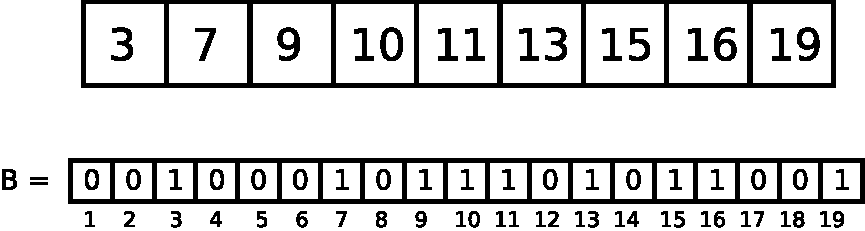
\includegraphics[scale=0.5]{bitmap.pdf}
\\\scriptsize{\color{white}.\color{black}\\Figura 7: Nodo mínimo en un BST}
\end{figure}
Para responder a las consultas predecesor y sucesor podemos usar las operaciones rank y select de los bitmaps:
\begin{itemize}
\item Sucesor: Select(B, Rank (B, i) + 1)
\begin{figure}[htp]
\centering
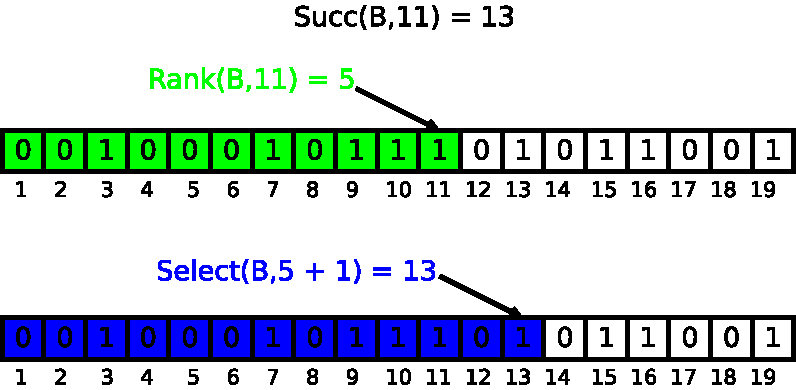
\includegraphics[scale=0.5]{bitmapsuc.pdf}
\\\scriptsize{\color{white}.\color{black}\\Figura 8: Ejemplo de sucesor con i = 11}
\end{figure}
\item Predecesor: Select(B, Rank (B, i $-$ 1))
\begin{figure}[htp]
\centering
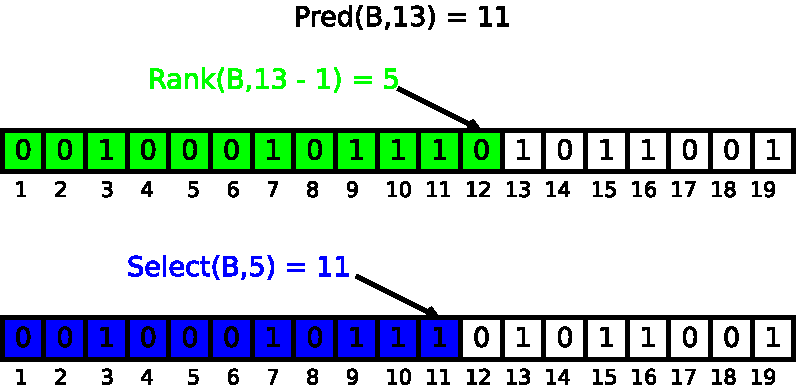
\includegraphics[scale=0.5]{bitmappred.pdf}
\\\scriptsize{\color{white}.\color{black}\\Figura 9: Ejemplo de predecesor con i = 11}
\end{figure}
\end{itemize}
\subsection{Análisis de complejidad de las soluciones}
\subsubsection{BST}
Las operaciones necesarias para obtener el predecesor y sucesor toman un tiempo que es proporcional a la altura del árbol. Para un BST con n nodos, las operaciones quedan acotadas a tiempos O(Log(n)) usando el método de análisis en el caso promedio y acotadas a tiempos O(n) usando el método de peor caso, cuando el árbol no está balanceado y hay que recorrer los nodos de manera secuencial.
\subsubsection{Bitmap}
Las únicas operaciones utilizadas en el bitmap son rank y select, las cuales pueden ser respondidas en tiempo constante O(1) utilizando bitmaps normales y también en tiempo O(k) para rank (k es la clave) y O(log n)  para select utilizando bitmaps H$_{0}$ - comprimidos, ambos ya implementados en la librería sdsl.
\subsection{Implementación de soluciones}
Se implementaron 3 clases en c++, BinarySearchTree, BitMap y BitMapH0, cada una de estas clases recibe como parámetro en su método constructor un vector de datos y a partir de este se inicializa cada estructura con dichos datos.

\subsubsection{BinarySearchTree}
Correspondiente a los archivos bst.cpp y bst.h, esta clase se implementó a partir de nodos que contienen un dato y punteros a sus hijos izquierdo, derecho y su nodo padre. La clase tiene guardada el nodo raíz y a partir del mismo se localiza el resto de los nodos.
\subsubsection{BitMap}
Corrrespondiente a los archivos bitmap.cpp y bitmap.h, esta clase se implementó a partir de la clase bit$\_$vector de la librería sdsl. La clase contiene un bit$\_$vector el cual tiene soporte de rank y select, métodos utilizados para obtener el predecesor y sucesor.
\subsubsection{BitMapH0}
Correspondiente a los archivos bitmap$\_$h0.cpp y bitmap$\_$h0.h, esta clase se implementó a partir de la clase rrr$\_$vector de la librería sdsl. Dicha clase corresponde a un bitmap H$_{0}$-comprimido y también tiene soporte de rank y select, ambos métodos utilizados de la misma forma que para BitMap, se podría decir que ambas clases son análogas.
\subsection{Dataset para los experimentos}
Para poder medir el tiempo de ejecutar la operación predecesor y sucesor, se utilizó un vector con \textbf{M} datos no repetidos, ordenados randómicamente en un rango \textbf{[1,N]}, con M = N / 2 en cada iteración. El valor de \textbf{M} disminuye a la mitad por cada iteración en un total de 8 iteraciones. El tamaño inicial del vector es de 8 Mb, siendo este incrementado hasta 1 Gb. Se utilizó el mismo vector para cada clase por iteración, solo cambiando este al comenzar una nueva iteración.
\subsection{Resultados experimentales}
\subsubsection{Formulación de hipótesis}
En base al análisis de complejidad de cada solución en el caso promedio, el bitmap debería ser más rápido, seguido por bitmap H$_{0}$-comprimido y finalmente el bst. 
\subsubsection{Experimento}
El siguiente experimento fué ejecutado en un computador con un procesador Intel Core i5 3230M (2600 MHz - 3200 MHz) con 12 Gb de memoria RAM. En cada iteración se ejecutó cada operación (predecesor y sucesor) 10.000 veces por cada clase sobre un elemento randómico distinto contenido en el vector original. Se midió el tiempo por cada operación y se calculó un promedió de las 10.000 operaciones distintas por cada clase.
\subsubsection{Resultados}
Luego de finalizada la ejecución del experimento se obtuvieron los siguientes resultados, con M medido en Mb y el tiempo promedio de cada operación medido en mili segundos.
\begin{center}\begin{tabular}{|l|c|c|c|c|c|c|}
\hline
	$M$ & $BST$ $pred$ & $BST$ $suc$ & $BM$ $pred$ & $BM$ $suc$ & $BMH_{0}$ $pred$ & $BMH_{0}$ $suc$ \\
\hline
8	&   1.3475	&   1.3522	&   0.4340 &	   0.4316 &	   1.0165 &	   0.9804 \\
\hline
16	&   1.3773	&   1.3798	&   0.4331 &	   0.4364 &	   0.9887 &	   0.9636 \\
\hline
32	&   1.6508	&   1.6432	&   0.4608 &	   0.4638 &	   1.0265 &	   0.9989 \\
\hline
64	&   1.9108	&   1.8856	&   0.5019 &	   0.5050 &	   1.0507 &	   1.0301 \\
\hline
128	 &  2.1253	&   2.1073	&   0.5466 &	   0.5527 &	   1.0985 &	   1.0647 \\
\hline
256	 &  2.3634	&   2.3445	&   0.5784 &	   0.5686 &	   1.2045 &	   1.1638 \\
\hline
512	 &  2.8431	&   2.8241	&   0.6605 &	   0.6470 &	   1.3886 &	   1.3410 \\
\hline
1024 &	   2.9252	&   2.9399	&   0.6229 &	   0.6148 &	   1.2804 &	   1.2132 \\ 
\hline
\end{tabular}
\\\scriptsize{\color{white}.\color{black}\\Figura 10: Tabla de resultados tiempo de ejecución algoritmos propuestos}
\end{center}
Para mejor visualización y análisis, se graficó los datos de la figura 10 en dos gráficos, uno para sucesor y otro para predecesor.
\begin{center}\begin{figure}[htp]
\centering
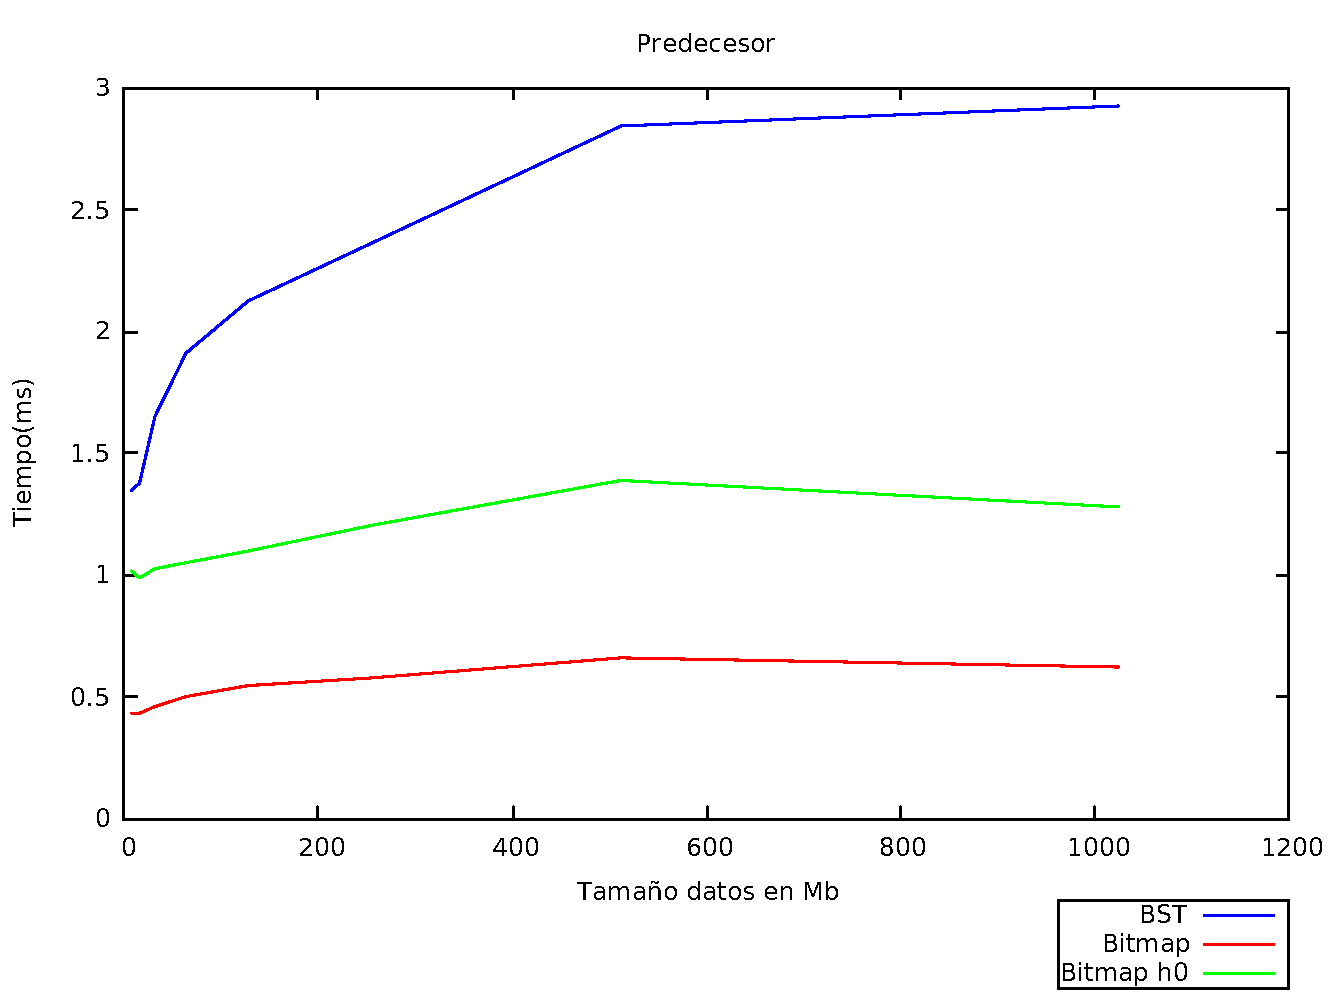
\includegraphics[scale=0.45]{exppred.pdf}
\\\scriptsize{\color{white}.\color{black}\\Figura 11: Comparación de soluciones para predecesor}
\label{etiqueta}
\end{figure}
\end{center}
\begin{center}\begin{figure}[htp]
\centering
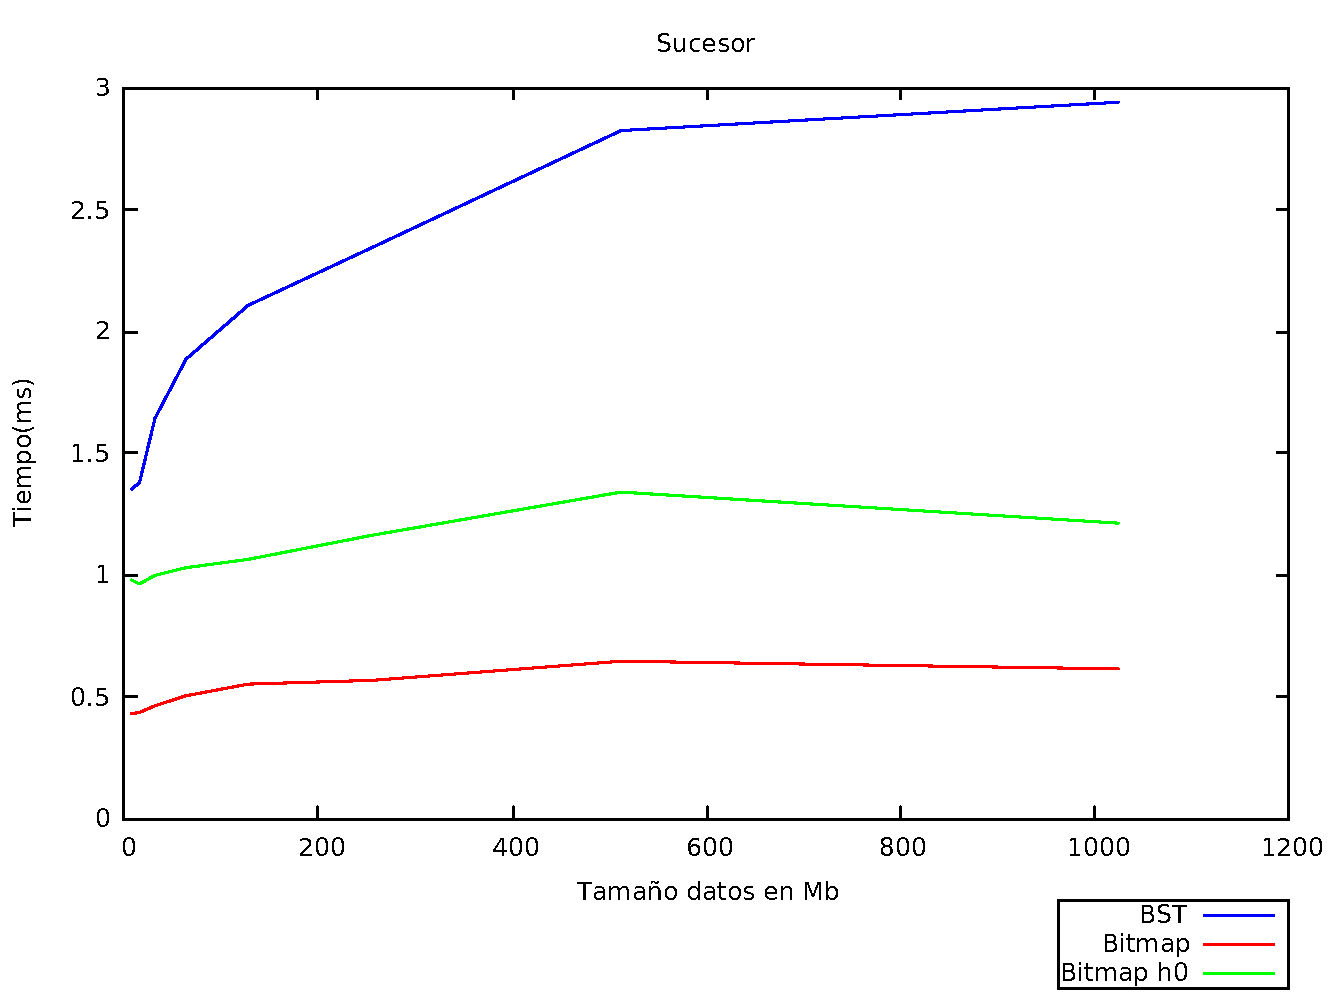
\includegraphics[scale=0.45]{expsuc.pdf}
\\\scriptsize{\color{white}.\color{black}\\Figura 12: Comparación de soluciones para sucesor}
\label{etiqueta}
\end{figure}
\end{center}
\clearpage
\subsubsection{Conclusión experimento}
Como podemos ver en la figura 11 y 12, los resultados obtenidos comprueban la hipótesis formulada al comienzo del experimento, para el cálculo del predecesor y sucesor el peor resultado obtenido fue la solución del BST. la curva de este tiene forma logarítmica. Para los bitmaps, el bitmap sin compresión obtuvo el mejor resultado.\\

Para el problema de predecesor y sucesor, la utilización de bitmaps presentó una mejora sobre el uso de binary search tree en términos de tiempo y espacio. El bitmap sin compresión es más rápido que su contraparte comprimida pero, evidentemente, gasta más espacio, por lo tanto la utilización de uno sobre otro depende de los requerimientos, si se debe priorizar tiempo por sobre espacio entonces es recomendable utilizar bitmap sin compresión, en el caso contrario es mejor utilizar bitmap H$_{0}$-comprimido.
\end{document}
